% ====================================================================================
\chapter{多智能体系统：从微观博弈到宏观平均场}
% ====================================================================================

% ====================================================================================
\section*{引言：当优化遇到博弈}
% ====================================================================================

\storynote{John Nash}{1928--2015，普林斯顿数学博士，21岁（1950年）就证明了纳什均衡的存在性。患精神分裂症数十年后奇迹康复，1994年获诺贝尔经济学奖。他的故事被拍成电影《美丽心灵》(A Beautiful Mind)，获奥斯卡最佳影片。2015年与妻子在出租车事故中去世。}

\storynote{John von Neumann}{1903--1957，20世纪最伟大的数学家之一，博弈论奠基人。他还发明了冯·诺伊曼计算机架构、参与曼哈顿计划、创立量子力学数学基础。据说他能用心算积分，智商估计超过180。}

在前面的章节中，我们一直在解决"一个智能体对抗环境"的问题：
\begin{itemize}
    \item 最优控制：一个控制器操控一个动力系统
    \item 强化学习：一个智能体在环境中最大化累积奖励
    \item PINN/神经算子：求解一个固定的PDE
\end{itemize}

但真实世界远比这复杂。想象以下场景：

\begin{quote}
\textit{早高峰时，每个司机都想选择最快的路线。但"最快"取决于其他人的选择——如果大家都选同一条路，这条路反而最慢。}
\end{quote}

\begin{quote}
\textit{在电力市场中，每个发电厂都想最大化利润。但电价取决于所有发电厂的总供应量——你的最优策略取决于别人怎么做。}
\end{quote}

\begin{quote}
\textit{一群无人机需要协作完成搜索任务。每架无人机的最优路径取决于其他无人机去哪里——你不想和别人重复搜索同一区域。}
\end{quote}

这些问题的共同特点是：\textbf{我的最优决策取决于你的决策，而你的最优决策也取决于我的决策}。

这就是\textbf{博弈论}（Game Theory）的领域。

\vspace{0.3cm}
\noindent\textit{为什么给城市多修一条路，反而可能让所有人都更堵？为什么"每个人都最优"和"整体最优"不是一回事？为什么当人多到数不清时，博弈论会变成流体力学？}

\begin{quote}
\textbf{本章目标}：当决策者不止一个时，"最优"这个词本身就要重新定义。本章要让你看到：纳什均衡不是新数学，而是把第1章的 KKT 条件同时写 $N$ 份；看似混乱的交通、市场和无人机群，背后常常藏着一个大家在共同最小化的势函数；而当玩家多到数不清时，博弈会自然地变成一对前向--后向的偏微分方程。
\end{quote}

\begin{tcolorbox}[colback=green!5, colframe=green!60!black, title=学完这章，你将能够...]
\begin{itemize}
    \item 用KKT条件计算简单博弈的纳什均衡
    \item 分析交通流量分配中的Wardrop均衡
    \item 理解QMIX、MAPPO等多智能体RL算法的核心思想
    \item 解释平均场博弈如何将$N$体问题简化为连续极限
    \item 用拉格朗日方法分析带约束的博弈问题
\end{itemize}
\end{tcolorbox}

% ====================================================================================
\section{博弈论基础：从优化到均衡}
% ====================================================================================

\subsection{从单人优化到多人博弈}

\review{第1章}{KKT 条件：驻点、可行、乘子非负、互补松弛。本章要做的只是把它写 $N$ 遍——每个玩家一遍——再要求它们同时成立。}
回顾单人优化问题：
\begin{equation}
    \min_{x} f(x) \quad \text{s.t.} \quad g(x) \leq 0
\end{equation}

最优解$x^*$满足KKT条件。这里只有一个决策者，目标函数$f(x)$只依赖于自己的决策$x$。

现在考虑\textbf{两人博弈}：

\begin{definition}[二人博弈]
一个二人博弈由以下元素组成：
\begin{itemize}
    \item \textbf{玩家1的策略空间}$\mathcal{A}_1$：玩家1可以选择的所有策略的集合
    \item \textbf{玩家2的策略空间}$\mathcal{A}_2$：玩家2可以选择的所有策略的集合
    \item \textbf{玩家1的代价函数}$J_1(a_1, a_2)$：玩家1要最小化的目标，\textbf{同时依赖于双方的策略}
    \item \textbf{玩家2的代价函数}$J_2(a_1, a_2)$：玩家2要最小化的目标，同样依赖于双方的策略
\end{itemize}
\end{definition}

\begin{remark}[与优化问题的关键区别]
在单人优化中，目标函数$f(x)$只依赖于决策者自己的选择$x$。但在博弈中，$J_1(a_1, a_2)$不仅依赖于玩家1的选择$a_1$，还依赖于玩家2的选择$a_2$。这意味着：
\begin{itemize}
    \item 玩家1想最小化$J_1$，但他控制不了$a_2$
    \item 玩家2想最小化$J_2$，但他控制不了$a_1$
    \item 双方的决策相互影响，形成一个"耦合"的系统
\end{itemize}
\end{remark}

每个玩家都想最小化自己的代价，但代价取决于对方的选择。这就产生了一个根本性的问题：

\begin{quote}
\textit{什么是"好"的策略组合？}
\end{quote}

\subsection{纳什均衡：没有人想单方面改变}
\review{第2章}{你其实已经见过纳什均衡：第2章把拉格朗日函数看成 $x$ 与 $\lambda$ 的零和博弈，强对偶成立时的鞍点 $(x^*, \lambda^*)$ 就是一个纳什均衡。}

\begin{definition}[纳什均衡]
策略组合$(a_1^*, a_2^*)$是一个\textbf{纳什均衡}（Nash Equilibrium），如果：
\begin{align}
    J_1(a_1^*, a_2^*) &\leq J_1(a_1, a_2^*), \quad \forall a_1 \in \mathcal{A}_1 \\
    J_2(a_1^*, a_2^*) &\leq J_2(a_1^*, a_2), \quad \forall a_2 \in \mathcal{A}_2
\end{align}
即：给定对方的策略，没有人能通过单方面改变自己的策略来降低代价。
\end{definition}

\begin{remark}[纳什均衡的直观理解]
让我们用更通俗的语言解释纳什均衡：

想象你和朋友在玩一个游戏。如果你们达到了纳什均衡状态，那意味着：
\begin{itemize}
    \item 你看了朋友的策略后，觉得"我现在的选择已经是最好的了，换别的只会更差"
    \item 你的朋友看了你的策略后，也觉得"我现在的选择已经是最好的了"
    \item 双方都没有动力去改变，系统达到一种"稳定"状态
\end{itemize}

\textbf{关键词}：单方面。纳什均衡不是说大家都开心，而是说没人想\textbf{单独}改变。
\end{remark}

\begin{example}[囚徒困境——博弈论最经典的例子]
\label{ex:prisoners}
两个囚犯分别被审讯，每人可以选择"合作"（保持沉默）或"背叛"（揭发对方）。

\textbf{变量含义}：
\begin{itemize}
    \item $a_1 \in \{\text{合作}, \text{背叛}\}$：玩家1的策略
    \item $a_2 \in \{\text{合作}, \text{背叛}\}$：玩家2的策略
    \item $J_1(a_1, a_2)$：玩家1的刑期（年），希望越小越好
    \item $J_2(a_1, a_2)$：玩家2的刑期（年），希望越小越好
\end{itemize}

代价矩阵（刑期）如下：

\begin{center}
\begin{tabular}{c|cc}
& 玩家2合作 & 玩家2背叛 \\
\hline
玩家1合作 & (1年, 1年) & (3年, 0年) \\
玩家1背叛 & (0年, 3年) & (2年, 2年) \\
\end{tabular}
\end{center}

\textbf{如何解读这个表格}：
\begin{itemize}
    \item 如果双方都合作（保持沉默），证据不足，各判1年
    \item 如果你背叛而对方合作，你当污点证人获释（0年），对方被重判（3年）
    \item 如果双方都背叛，各判2年
\end{itemize}

\textbf{分析纳什均衡}——我们来做"最优响应分析"：

\textit{假设玩家2选择合作}：
\begin{itemize}
    \item 玩家1选合作：刑期1年
    \item 玩家1选背叛：刑期0年 $\leftarrow$ \textbf{更好！}
\end{itemize}

\textit{假设玩家2选择背叛}：
\begin{itemize}
    \item 玩家1选合作：刑期3年
    \item 玩家1选背叛：刑期2年 $\leftarrow$ \textbf{更好！}
\end{itemize}

结论：\textbf{无论玩家2怎么选，玩家1选背叛总是更好}。这叫做"背叛是玩家1的\textbf{占优策略}"。

由于博弈是对称的，玩家2也会得出同样结论。

因此，\textbf{（背叛，背叛）是唯一的纳什均衡}，双方各判2年。

\textbf{悖论所在}：如果双方都选合作，各判1年，明明对双方都更好！但理性的个体不会选择合作，因为背叛总是对自己更有利。

这揭示了博弈论的一个深刻洞察：\textbf{个体理性不一定导致集体理性}。
\end{example}
\think{如果两人可以事先签一份"背叛者赔付 3 年"的合同，代价矩阵会怎样变？新的纳什均衡在哪里？（提示：合同就是一条新约束。）}

\begin{figure}[htbp]
\centering
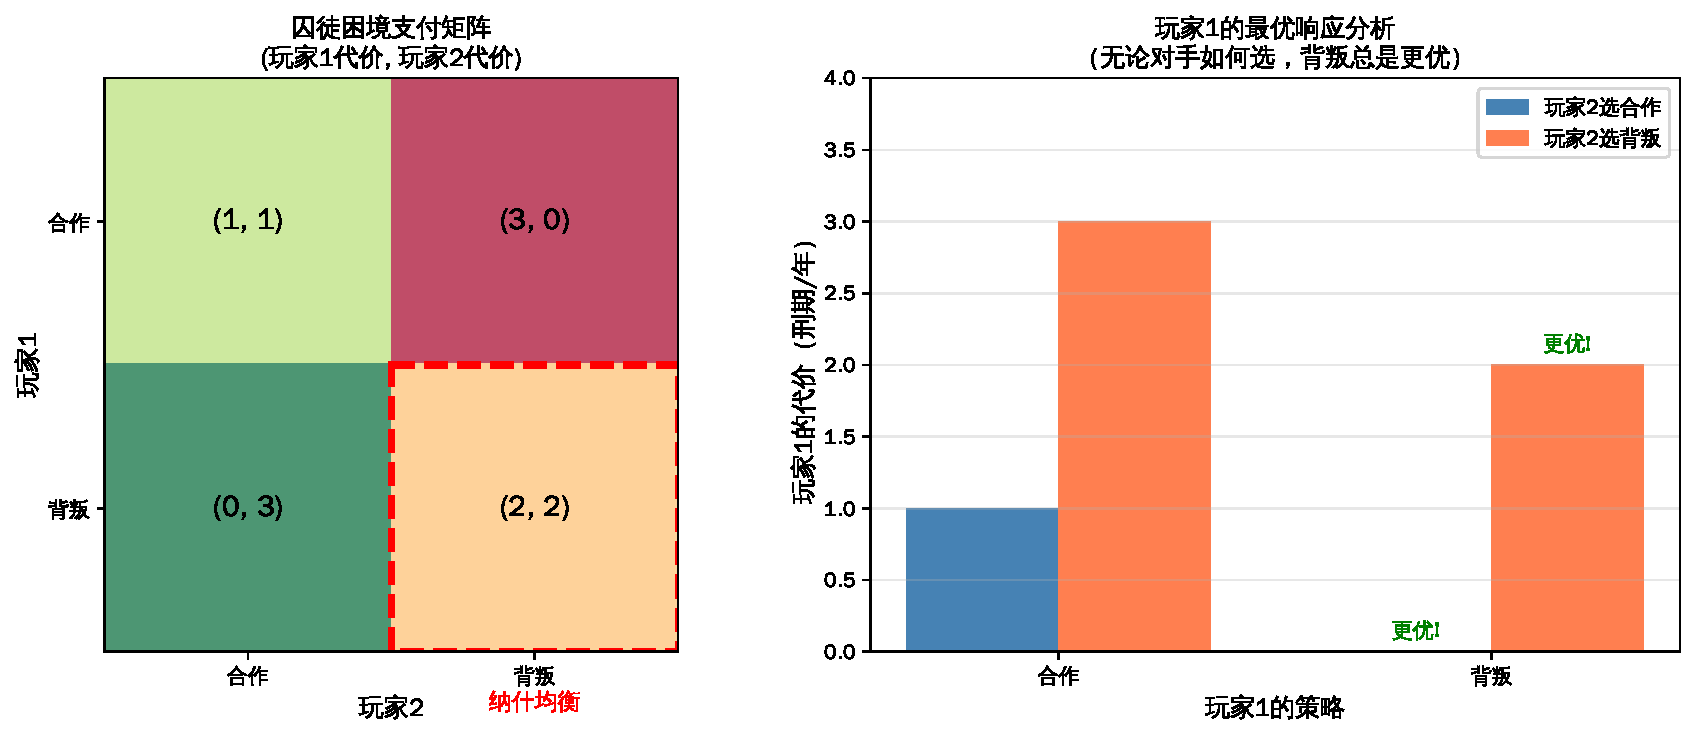
\includegraphics[width=0.95\textwidth]{figs_chap15/prisoners_dilemma.pdf}
\caption{囚徒困境的可视化分析。左图：支付矩阵热力图，红色虚线框标记纳什均衡（背叛，背叛）。右图：玩家1的最优响应分析，无论玩家2如何选择，背叛都是玩家1的更优选择。}
\label{fig:prisoners}
\end{figure}

图\ref{fig:prisoners}展示了囚徒困境的两种分析视角。从右图可以清楚看到：不管对手选什么，选择背叛总能让自己的代价更低。这就是为什么理性的玩家会陷入（背叛，背叛）的均衡，尽管（合作，合作）对双方都更好。

\subsection{连续策略博弈与最优响应}

当策略空间是连续的（如$\mathcal{A}_i = \R$），我们可以用微积分来分析。

\begin{definition}[最优响应]
给定对手的策略$a_{-i}$，玩家$i$的\textbf{最优响应}（Best Response）是：
\begin{equation}
    BR_i(a_{-i}) = \arg\min_{a_i \in \mathcal{A}_i} J_i(a_i, a_{-i})
\end{equation}

\textbf{直观理解}：如果我知道对手会选$a_{-i}$，我应该选什么来最小化自己的代价？答案就是$BR_i(a_{-i})$。
\end{definition}

\begin{proposition}[纳什均衡的不动点特征]
$(a_1^*, a_2^*)$是纳什均衡，当且仅当：
\begin{equation}
    a_1^* = BR_1(a_2^*), \quad a_2^* = BR_2(a_1^*)
\end{equation}
即每个人的策略都是对方策略的最优响应。
\end{proposition}

\begin{remark}[不动点的直观含义]
这个条件说的是：在纳什均衡点，形成了一个"自洽"的循环：
\begin{itemize}
    \item 玩家1选$a_1^*$是因为对手选了$a_2^*$
    \item 玩家2选$a_2^*$是因为对手选了$a_1^*$
    \item 谁也不想先改变，因为改变只会让自己更差
\end{itemize}

这正是数学中"不动点"的概念：$x^* = f(x^*)$，即函数作用在某个点上还是它自己。
\end{remark}

这给出了一个寻找纳什均衡的算法思路：\textbf{迭代最优响应}（Iterated Best Response）。

\begin{algorithm}
\caption{迭代最优响应（伪代码）}
\begin{algorithmic}[1]
\State \textbf{输入}: 初始策略 $a_1^{(0)}, a_2^{(0)}$，迭代次数 $K$
\State \textbf{输出}: 近似纳什均衡 $(a_1^{(K)}, a_2^{(K)})$
\For{$k = 0, 1, 2, \ldots, K-1$}
    \State $a_1^{(k+1)} \leftarrow BR_1(a_2^{(k)})$ \Comment{玩家1对玩家2当前策略的最优响应}
    \State $a_2^{(k+1)} \leftarrow BR_2(a_1^{(k+1)})$ \Comment{玩家2对玩家1新策略的最优响应}
\EndFor
\State \Return $(a_1^{(K)}, a_2^{(K)})$
\end{algorithmic}
\end{algorithm}

\begin{warning}[title=迭代最优响应不一定收敛]
迭代最优响应可能：
\begin{itemize}
    \item \textbf{收敛到纳什均衡}（如果博弈是"好"的）
    \item \textbf{陷入循环}（如石头剪刀布）
    \item \textbf{发散}
\end{itemize}
收敛性取决于博弈的结构，我们稍后会看到一类保证收敛的"势博弈"。
\end{warning}
\preview{下一节的 Beckmann 势函数就是这样的例子：每个司机各自为政，宏观上却在最小化同一个凸函数 $\Phi$——博弈又变回了第1章的优化。}

% ====================================================================================
\section{物理约束下的静态博弈}
% ====================================================================================

\begin{tcolorbox}[colback=yellow!10, colframe=orange!80, title=本章的核心观点]
\textbf{本章的问题就是第1章的拉格朗日乘子法，只是要同时写 $N$ 份——每个玩家一份，各自只对自己的变量求导，却共享同一组变量。}

这不是比喻：广义纳什均衡的定义，就是"$N$ 组 KKT 条件同时成立"。

\begin{center}
\renewcommand{\arraystretch}{1.3}
\small
\begin{tabular}{lll}
\toprule
\textbf{概念} & \textbf{第1章（单人优化）} & \textbf{本章（博弈）} \\
\midrule
变量 & 一个向量 $x$ & $N$ 个玩家各自的 $a_i$，合起来 $(a_1, \ldots, a_N)$ \\
目标 & 一个 $f(x)$ & $N$ 个 $J_i(a_i, a_{-i})$，玩家 $i$ 只管自己的 \\
约束 & $g(x) \le 0$ & $g_i(a_i, a_{-i}) \le 0$，可能依赖别人的选择 \\
乘子 & $\lambda$：影子价格 & 每人一组 $\lambda_i$；Wardrop 中 $\lambda_w$ = 均衡旅行时间 \\
一阶条件 & 一组 KKT & $N$ 组 KKT 同时成立 $=$ 广义纳什均衡 \\
特例 & --- & 势博弈：$N$ 组 KKT 恰好是同一个 $\Phi$ 的一组 KKT \\
\bottomrule
\end{tabular}
\end{center}
\end{tcolorbox}

\subsection{广义纳什均衡与KKT条件}

在实际问题中，每个玩家的策略通常受到\textbf{物理约束}：
\begin{itemize}
    \item 能量上限：$\|a_i\|^2 \leq E_{\max}$
    \item 位置限制：$a_i \in [0, L]$
    \item 资源预算：$c^T a_i \leq B$
\end{itemize}

\begin{definition}[广义纳什均衡问题]
$N$个玩家的\textbf{广义纳什均衡问题}（Generalized Nash Equilibrium Problem, GNEP）：

每个玩家$i$求解：
\begin{equation}
    \min_{a_i} J_i(a_i, a_{-i}) \quad \text{s.t.} \quad g_i(a_i, a_{-i}) \leq 0
\end{equation}

\textbf{变量说明}：
\begin{itemize}
    \item $a_i$：玩家$i$的策略（决策变量）
    \item $a_{-i}$：除玩家$i$外所有其他玩家的策略
    \item $J_i$：玩家$i$的代价函数
    \item $g_i$：玩家$i$面临的约束（可能依赖于其他玩家的策略）
\end{itemize}
\end{definition}

\begin{keyinsight}
纳什均衡可以用\textbf{KKT条件系统}来刻画！

在纳什均衡$(a_1^*, \ldots, a_N^*)$处，每个玩家$i$的策略$a_i^*$必须满足其优化问题的KKT条件：
\begin{align}
    \nabla_{a_i} J_i(a_i^*, a_{-i}^*) + \sum_j \lambda_{ij}^* \nabla_{a_i} g_{ij}(a_i^*, a_{-i}^*) &= 0 \quad \text{（驻点条件）} \\
    \lambda_{ij}^* &\geq 0 \quad \text{（乘子非负）} \\
    \lambda_{ij}^* g_{ij}(a_i^*, a_{-i}^*) &= 0 \quad \text{（互补松弛）} \\
    g_{ij}(a_i^*, a_{-i}^*) &\leq 0 \quad \text{（可行性）}
\end{align}

这是$N$组KKT条件\textbf{同时成立}！
\end{keyinsight}
\clarify{单人优化是"一个目标、一组 KKT"；博弈是"$N$ 个目标、$N$ 组 KKT"，它们共享变量，却各自只对自己的 $a_i$ 求导。所以均衡一般不是任何一个函数的极小点——除非它是势博弈。}

\begin{remark}[KKT条件的物理意义]
回忆一下KKT条件的含义：
\begin{itemize}
    \item \textbf{驻点条件}：在最优点，目标函数的梯度被约束的梯度"抵消"了
    \item \textbf{互补松弛}：约束要么不起作用（$g < 0$），要么起作用但乘子为正（$\lambda > 0$）
\end{itemize}

在博弈中，每个玩家都在自己的约束下做优化，所以每个人的KKT条件都要满足。纳什均衡就是这$N$组条件的公共解。
\end{remark}

\subsection{案例一：图博弈——邻居之间的互动}

\begin{definition}[图博弈]
在\textbf{图博弈}（Network Game）中：
\begin{itemize}
    \item 玩家位于图$G = (V, E)$的节点上
    \item 玩家$i$的代价只依赖于自己和\textbf{邻居}的策略：
    \begin{equation}
        J_i(a_i, a_{N(i)}) = f_i(a_i) + \sum_{j \in N(i)} \phi_{ij}(a_i, a_j)
    \end{equation}
    其中$N(i)$是$i$的邻居集合
\end{itemize}
\end{definition}

\begin{example}[线性二次图博弈——一个完整的求解过程]
\label{ex:lq_network}
考虑代价函数：
\begin{equation}
    J_i = \frac{1}{2}(a_i - a_{i,0})^2 + \delta \cdot a_i \sum_{j \in N(i)} a_j
\end{equation}

\textbf{变量含义详解}：
\begin{itemize}
    \item $a_i \in \R$：玩家$i$的策略/行动（比如生产量、投入的努力等）
    \item $a_{i,0}$：玩家$i$的"理想状态"或"目标值"（如果没有邻居影响，他想选择的值）
    \item $\delta$：交互强度参数，决定邻居对你的影响有多大
    \item $N(i)$：玩家$i$的邻居集合（图中与$i$相连的节点）
\end{itemize}

\textbf{代价函数的物理解释}：
\begin{itemize}
    \item \textbf{第一项} $(a_i - a_{i,0})^2/2$：偏离理想状态的代价。你想待在$a_{i,0}$附近，离得越远代价越大
    \item \textbf{第二项} $\delta \cdot a_i \sum_{j \in N(i)} a_j$：与邻居的交互代价
    \begin{itemize}
        \item 如果$\delta > 0$（\textbf{策略替代}）：邻居做得多，你做得多会增加代价。类似于竞争关系——市场上对手生产越多，你再多生产就越亏
        \item 如果$\delta < 0$（\textbf{策略互补}）：邻居做得多，你做得多反而减少代价。类似于协作关系——朋友都在学习，你学习效果也更好
    \end{itemize}
\end{itemize}

\textbf{求解纳什均衡}：

每个玩家$i$想最小化$J_i$，将$a_i$视为决策变量，$a_{-i}$视为已知。

对$a_i$求导并令其为零（一阶最优性条件）：
\begin{equation}
    \frac{\partial J_i}{\partial a_i} = (a_i - a_{i,0}) + \delta \sum_{j \in N(i)} a_j = 0
\end{equation}

解这个方程得到\textbf{最优响应}：
\begin{equation}
    a_i^* = a_{i,0} - \delta \sum_{j \in N(i)} a_j^*
\end{equation}

\textbf{解读}：如果$\delta > 0$（竞争），邻居行动越大，你的最优响应越小。如果$\delta < 0$（协作），邻居行动越大，你也应该行动更大。

\textbf{矩阵形式}：

把所有$N$个玩家的最优响应方程写在一起：
\begin{equation}
    \mathbf{a}^* = \mathbf{a}_0 - \delta A \mathbf{a}^*
\end{equation}
其中$A$是图的邻接矩阵：$A_{ij} = 1$如果$i$和$j$是邻居，否则为0。

移项整理：
\begin{equation}
    (I + \delta A) \mathbf{a}^* = \mathbf{a}_0
\end{equation}

解得纳什均衡：
\begin{equation}
    \boxed{\mathbf{a}^* = (I + \delta A)^{-1} \mathbf{a}_0}
\end{equation}

这是一个漂亮的闭式解！只需要知道图结构（邻接矩阵$A$）和每个人的理想状态（$\mathbf{a}_0$），就能直接算出均衡。
\tryit{用 NumPy 构造 6 节点环形图的邻接矩阵，分别取 $\delta = 0.15$ 和 $\delta = 0.6$ 计算 $(I + \delta A)^{-1}\mathbf{a}_0$，再跑迭代最优响应。哪个 $\delta$ 下迭代发散？和 $A$ 的谱半径比一比。}
\end{example}

\begin{figure}[htbp]
\centering
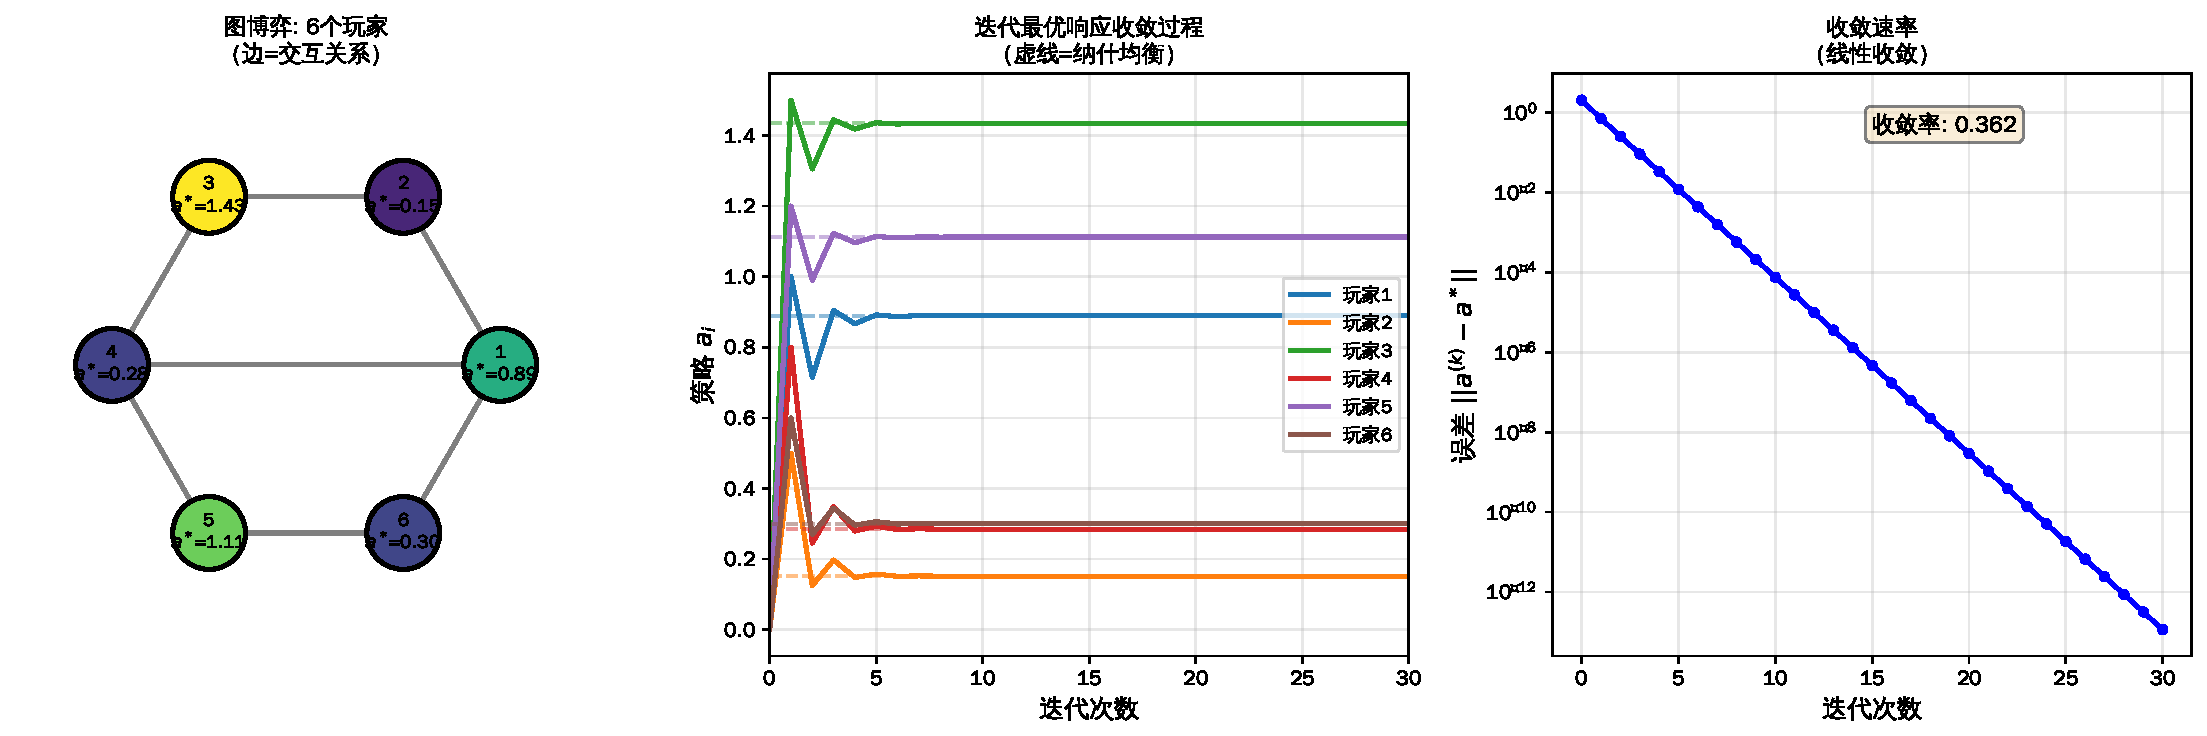
\includegraphics[width=0.95\textwidth]{figs_chap15/network_game.pdf}
\caption{图博弈的数值实验。左图：6个玩家组成的网络，节点颜色表示均衡策略的大小。中图：迭代最优响应过程，从零初始化出发，每个玩家的策略逐渐收敛到纳什均衡（虚线）。右图：收敛误差随迭代次数呈指数下降，表明算法线性收敛。参数：$\delta = 0.15$（策略替代）。}
\label{fig:network_game}
\end{figure}

图\ref{fig:network_game}展示了图博弈的实际计算结果。可以观察到：
\begin{itemize}
    \item 迭代最优响应算法确实收敛到了纳什均衡
    \item 收敛速度是\textbf{线性}的（在对数坐标下误差直线下降）
    \item 不同位置的玩家（中心节点vs边缘节点）有不同的均衡策略
\end{itemize}

\subsection{案例二：交通均衡与Braess悖论}

\begin{example}[Wardrop交通均衡]
\label{ex:wardrop}
考虑一个交通网络：
\begin{itemize}
    \item $W$个OD对（Origin-Destination，起点-终点对）
    \item 每个OD对$w$有需求$d_w$（单位时间内要从起点到终点的车辆数）
    \item 每个OD对有多条可选路径$P_w$
    \item 每条边$a$有时间函数$t_a(x_a)$，其中$x_a$是边$a$的流量
\end{itemize}

\textbf{Wardrop第一原理}（用户均衡）：在均衡状态下，每个OD对所有被使用的路径具有\textbf{相同且最小}的旅行时间。

\textbf{直观理解}：如果有一条更快的路，司机会切换过去。切换的人多了，那条路就变慢了。最终达到平衡：所有在用的路一样快，没人想换。
\end{example}

\begin{example}[Braess悖论——增加道路反而更堵！]
\label{ex:braess}
\storynote{Dietrich Braess}{德国数学家（1938--）。1968 年他研究交通网络的数值方法时发现：给路网加一条边，可能让所有人的均衡旅行时间变长。这篇德语论文沉寂多年，直到规划者在纽约、首尔的真实道路上看到同样现象才广为人知。}
这是交通领域最著名的悖论之一。考虑从起点S到终点E的交通网络：

\textbf{网络结构}：
\begin{itemize}
    \item 节点：S（起点）、A、B、E（终点）
    \item 边SA：时间函数$t_{SA}(x) = x/100$（流量越大越慢）
    \item 边AE：固定时间$t_{AE} = 45$分钟
    \item 边SB：固定时间$t_{SB} = 45$分钟
    \item 边BE：时间函数$t_{BE}(x) = x/100$
    \item 边AB（Braess边）：时间$t_{AB} = 0$（\textbf{免费捷径！}）
\end{itemize}

总需求：4000辆车从S到E。

\textbf{情况1：没有AB边}

可选路径：
\begin{itemize}
    \item 路径1：S $\to$ A $\to$ E，时间 = $x_{SA}/100 + 45$
    \item 路径2：S $\to$ B $\to$ E，时间 = $45 + x_{BE}/100$
\end{itemize}

由对称性，均衡时各2000辆车：
\begin{itemize}
    \item 路径1时间：$2000/100 + 45 = 20 + 45 = 65$分钟
    \item 路径2时间：$45 + 2000/100 = 45 + 20 = 65$分钟 $\checkmark$
\end{itemize}

\textbf{所有人旅行时间：65分钟}

\textbf{情况2：有AB边（免费捷径）}

新增路径3：S $\to$ A $\to$ B $\to$ E，时间 = $x_{SA}/100 + 0 + x_{BE}/100$

\textbf{关键分析}：假设所有4000辆车都走路径3（S$\to$A$\to$B$\to$E）：
\begin{itemize}
    \item 路径3时间：$4000/100 + 0 + 4000/100 = 40 + 0 + 40 = 80$分钟
\end{itemize}

验证这是纳什均衡——有人想换路吗？
\begin{itemize}
    \item 换到路径1（S$\to$A$\to$E）：$40 + 45 = 85$分钟 > 80分钟，更差！
    \item 换到路径2（S$\to$B$\to$E）：$45 + 40 = 85$分钟 > 80分钟，更差！
\end{itemize}

没人想换，所以\textbf{所有人走S$\to$A$\to$B$\to$E确实是纳什均衡}。

\textbf{所有人旅行时间：80分钟}

\textbf{悖论}：增加了一条\textbf{免费}道路，所有人的旅行时间反而从65分钟增加到80分钟！增加了约23\%！

\textbf{为什么会这样？}
\begin{itemize}
    \item 免费捷径看起来很诱人
    \item 每个人都"理性"地选择它
    \item 但大家都这么想，导致SA和BE两条边都拥挤了
    \item 如果政府\textbf{禁止}这条免费道路，反而能让所有人更快到达！
\end{itemize}

这再次说明：\textbf{个体理性 $\neq$ 集体理性}。
\end{example}

\begin{figure}[htbp]
\centering
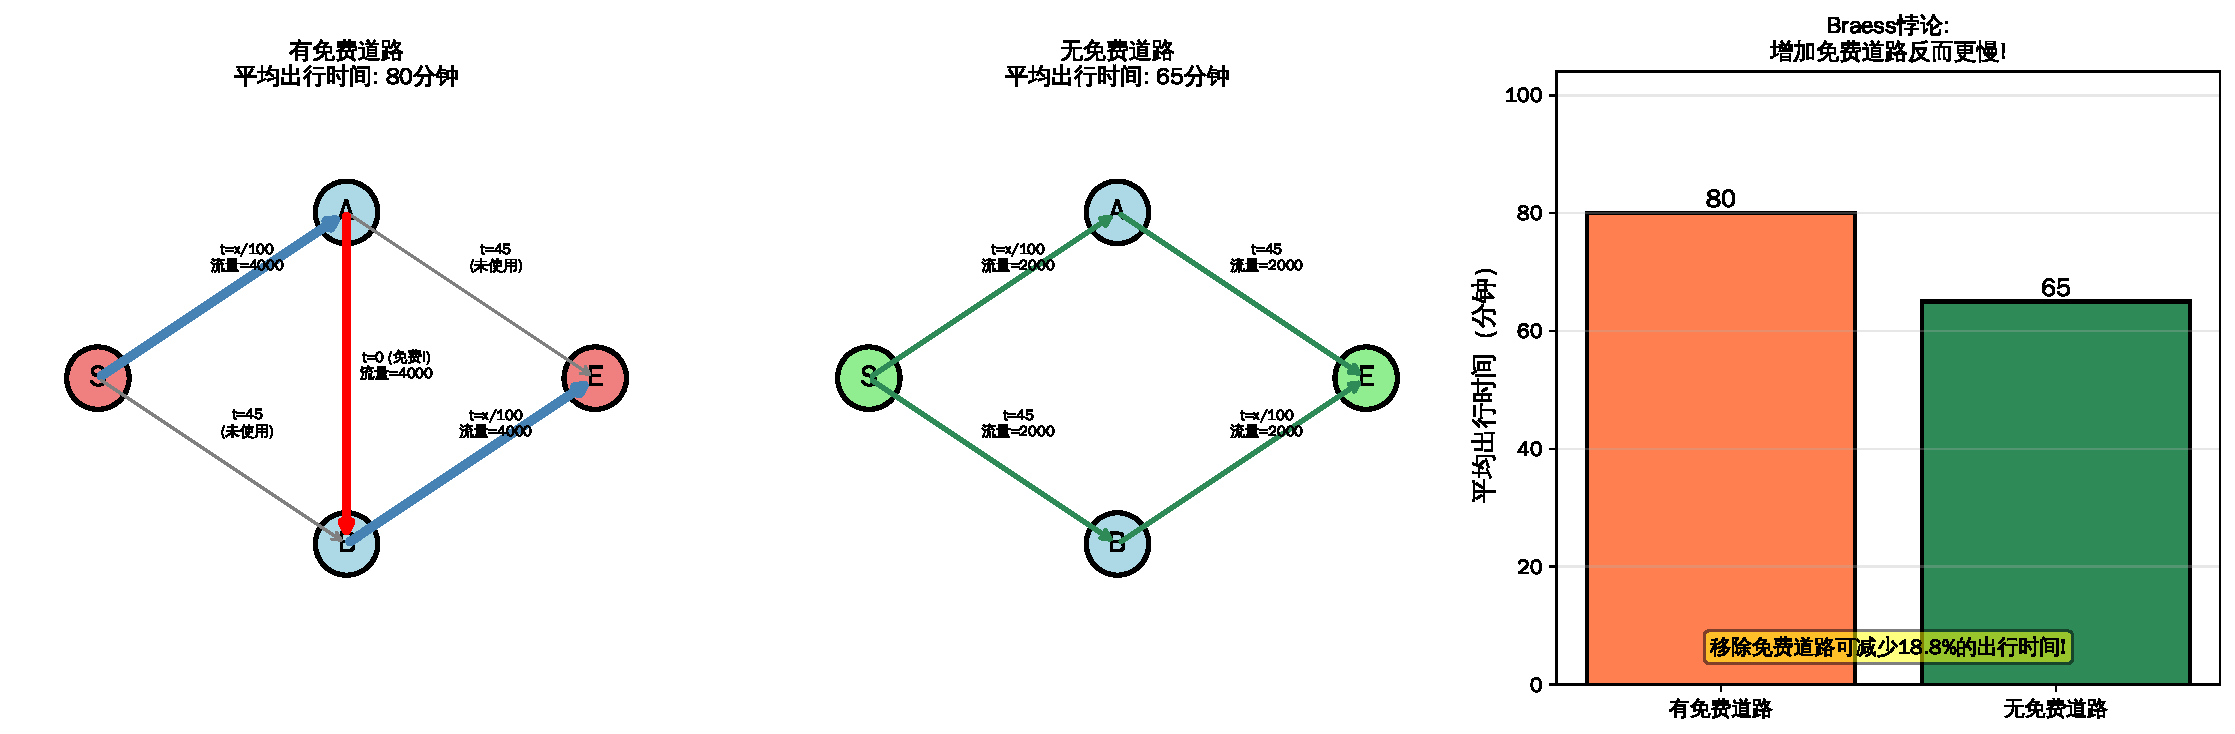
\includegraphics[width=0.95\textwidth]{figs_chap15/braess_paradox.pdf}
\caption{Braess悖论的数值验证。左图：有免费道路（红色AB边）时，所有车辆都选择S$\to$A$\to$B$\to$E路径，平均旅行时间80分钟。中图：没有免费道路时，车辆均匀分布在两条路径上，平均旅行时间65分钟。右图：柱状对比显示，移除免费道路可减少约18.8\%的旅行时间。}
\label{fig:braess}
\end{figure}

图\ref{fig:braess}直观展示了Braess悖论。这个悖论在现实中确实存在——1990年代，纽约市关闭了第42街的一段道路后，周围的交通状况反而改善了！首尔在2003年拆除了一条高架路后，交通拥堵也得到缓解。

\subsection{势博弈：自私博弈的隐藏秩序}

\begin{theorem}[Beckmann势函数]
如果边时间函数$t_a(x_a)$是连续且非递减的，则Wardrop用户均衡是以下\textbf{凸优化问题}的解：
\begin{equation}
    \min_{\mathbf{f}} \Phi(\mathbf{x}(\mathbf{f})) = \sum_{a} \int_0^{x_a} t_a(s) \, ds
\end{equation}
\begin{equation}
    \text{s.t.} \quad \sum_{p \in P_w} f_p = d_w, \quad f_p \geq 0, \quad x_a = \sum_{p \ni a} f_p
\end{equation}

\textbf{变量说明}：
\begin{itemize}
    \item $f_p$：路径$p$上的流量
    \item $x_a$：边$a$上的总流量（所有经过边$a$的路径流量之和）
    \item $d_w$：OD对$w$的总需求
    \item $\Phi$：Beckmann势函数
\end{itemize}
\end{theorem}

\begin{proof}[用KKT条件证明Wardrop均衡]
这是一个经典的``优化 $\Leftrightarrow$ 均衡''对应。让我们用KKT条件来证明Beckmann问题的解恰好满足Wardrop用户均衡条件。

\textbf{Step 1：写出拉格朗日函数}

对于路径流量$f_p$的约束优化问题，拉格朗日函数为：
\begin{equation}
    \mathcal{L} = \sum_{a} \int_0^{x_a} t_a(s) \, ds - \sum_w \lambda_w \left( \sum_{p \in P_w} f_p - d_w \right) - \sum_p \mu_p f_p
\end{equation}
其中：
\begin{itemize}
    \item $\lambda_w$：OD对$w$的需求约束的乘子
    \item $\mu_p \geq 0$：路径流量非负约束$f_p \geq 0$的乘子
\end{itemize}
（这里把 $f_p \ge 0$ 写成 $-f_p \le 0$，并用减号引入乘子；与第1章的 $\Lag = f + \lambda g + \mu h$ 只差记号约定。）

\textbf{Step 2：对$f_p$求偏导}

注意$x_a = \sum_{p \ni a} f_p$，所以$\frac{\partial x_a}{\partial f_p} = 1$（如果路径$p$经过边$a$）。因此：
\begin{equation}
    \frac{\partial \mathcal{L}}{\partial f_p} = \sum_{a \in p} t_a(x_a) - \lambda_w - \mu_p = 0
\end{equation}
即：\textbf{路径$p$的总旅行时间} = $\lambda_w + \mu_p$

\textbf{Step 3：互补松弛条件}

KKT的互补松弛条件要求：$\mu_p \cdot f_p = 0$
\begin{itemize}
    \item 若$f_p > 0$（路径被使用），则$\mu_p = 0$，故路径时间 $= \lambda_w$
    \item 若$f_p = 0$（路径未被使用），则$\mu_p \geq 0$，故路径时间 $\geq \lambda_w$
\end{itemize}

\textbf{Step 4：这正是Wardrop条件！}

上述结论可以总结为：
\begin{center}
\fbox{\parbox{0.8\textwidth}{
\textbf{所有被使用的路径}（$f_p > 0$）具有\textbf{相同的}旅行时间$\lambda_w$；\\
\textbf{所有未被使用的路径}（$f_p = 0$）旅行时间$\geq \lambda_w$。
}}
\end{center}

这正是Wardrop第一原理的数学表述！乘子$\lambda_w$就是OD对$w$的\textbf{均衡旅行时间}。
\end{proof}
\clarify{这正是第1章的影子价格：$\partial \Phi^*/\partial d_w = \lambda_w$，再多派一辆车走 OD 对 $w$，势函数恰好增加这辆车自己经历的旅行时间。它不等于系统总旅行时间的增量——后者还要加上这辆车给别人添的堵，两者之差 $x_a t_a'(x_a)$ 就是"拥堵费"。}

\begin{keyinsight}
\textbf{自私博弈的隐藏秩序}：

看似混乱的交通系统——每个司机都在自私地最小化自己的旅行时间——在宏观上却等价于在优化一个系统的``总势能''$\Phi$。

这类博弈被称为\textbf{势博弈}（Potential Game）：存在一个势函数$\Phi$，每个玩家改变策略导致的代价变化等于势函数的变化。

势博弈有很好的性质：
\begin{itemize}
    \item 纳什均衡一定存在（$\Phi$的最小值点）
    \item 最优响应动态一定收敛（因为$\Phi$单调下降）
    \item 可以用优化算法求解均衡
\end{itemize}
\end{keyinsight}

\begin{figure}[htbp]
\centering
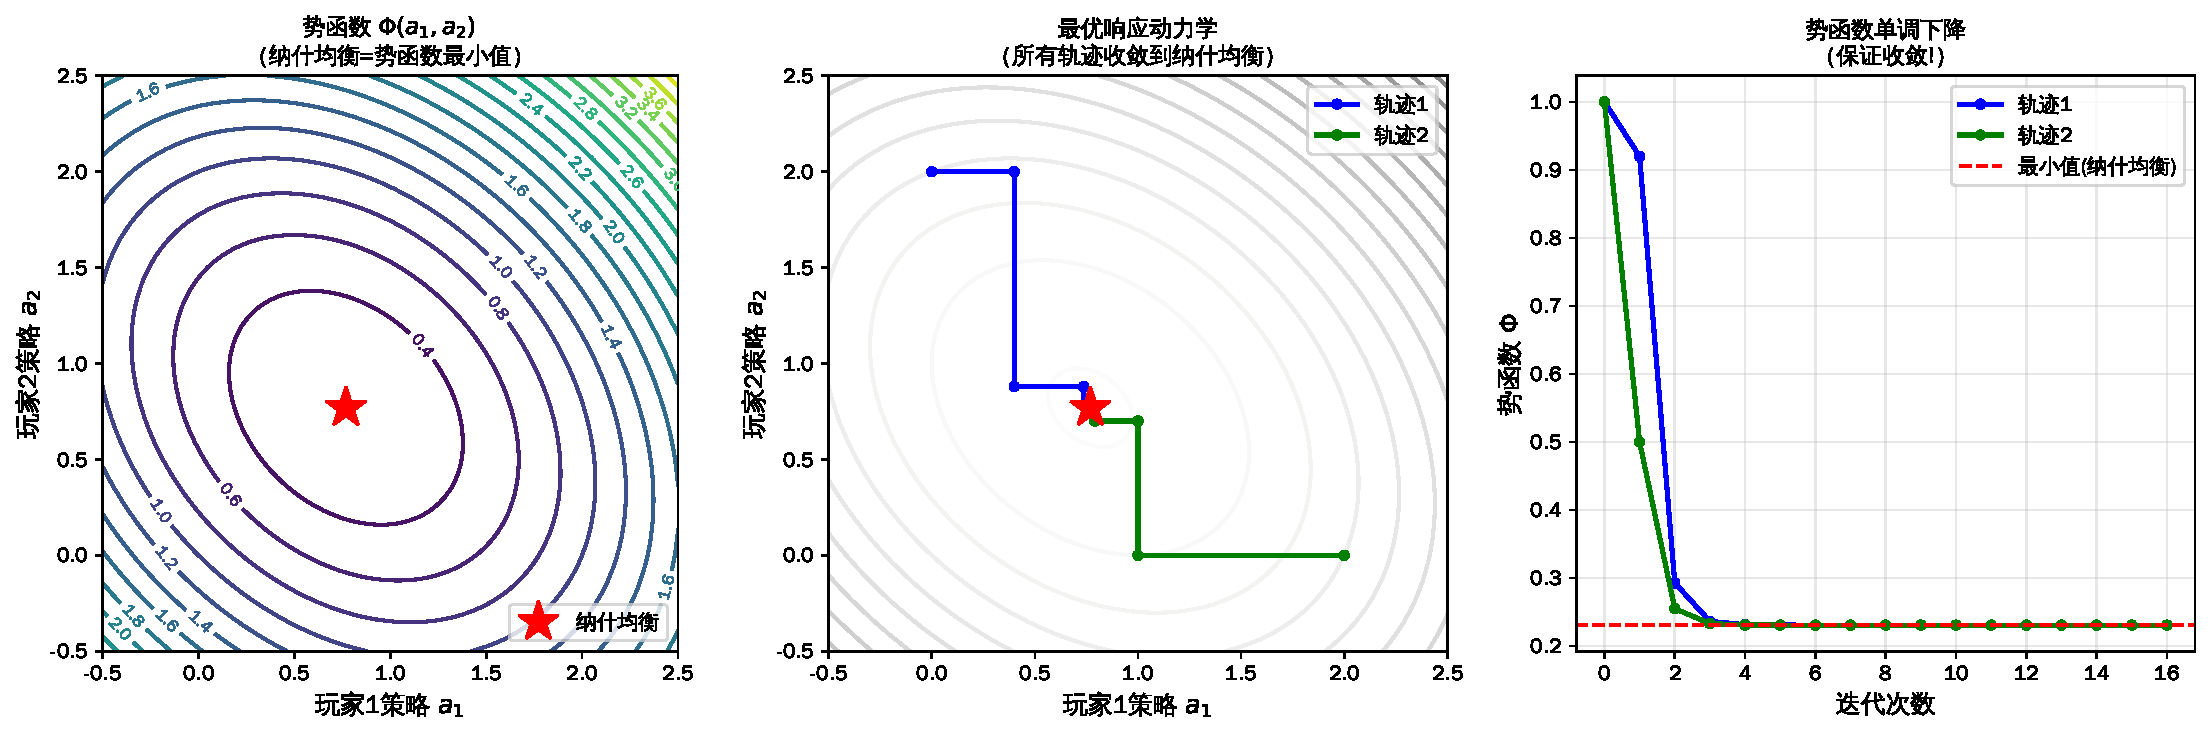
\includegraphics[width=0.95\textwidth]{figs_chap15/potential_game.pdf}
\caption{势博弈的收敛性质。左图：势函数$\Phi(a_1, a_2)$的等高线，红星标记纳什均衡（势函数最小值点）。中图：从不同初始点出发的迭代最优响应轨迹，都收敛到纳什均衡。右图：势函数沿轨迹单调下降，保证收敛性。}
\label{fig:potential}
\end{figure}

图\ref{fig:potential}展示了势博弈的核心性质：势函数沿着迭代最优响应的轨迹\textbf{单调下降}。这就像一个小球在山谷中滚动，总会滚到最低点（纳什均衡）。这也是为什么势博弈特别"好"——我们可以把博弈问题转化为优化问题来求解。

% ====================================================================================
\section{深度多智能体强化学习}
% ====================================================================================

前面我们讨论的都是\textbf{静态博弈}——玩家同时做出决策，博弈只进行一轮。

现在我们加入\textbf{时间}维度：智能体需要在多个时间步做出决策，当前决策会影响未来状态。这就是\textbf{动态博弈}，或更具体地说，\textbf{马尔可夫博弈}（Markov Game）。

\subsection{从静态到动态：马尔可夫博弈}

\begin{definition}[马尔可夫博弈]
一个$N$人\textbf{马尔可夫博弈}（又称随机博弈）由以下元素组成：
\begin{itemize}
    \item \textbf{状态空间}$\mathcal{S}$：系统可能处于的所有状态
    \item \textbf{动作空间}$\mathcal{A}_i$：每个智能体$i$可选择的动作
    \item \textbf{状态转移}$P(s' | s, a_1, \ldots, a_N)$：给定当前状态和所有人的动作，下一个状态的概率分布
    \item \textbf{奖励函数}$r_i(s, a_1, \ldots, a_N)$：每个智能体在每一步获得的即时奖励
    \item \textbf{折扣因子}$\gamma \in [0,1)$：未来奖励的折扣率
\end{itemize}

每个智能体$i$的目标是最大化累积奖励：
\begin{equation}
    \max_{\pi_i} \E\left[ \sum_{t=0}^{\infty} \gamma^t r_i(s_t, a_{1,t}, \ldots, a_{N,t}) \right]
\end{equation}
\end{definition}

\review{第10章}{第10章里 Q 学习、策略梯度的收敛性都假设转移概率固定。这里 $\pi_{-i}$ 在变，等于地基在动——单智能体的收敛保证从根上失效。}
\begin{warning}[title=多智能体RL的核心困难：非平稳性]
\textbf{问题}：从智能体$i$的视角看，环境的转移概率是：
\begin{equation}
    P(s' | s, a_i) = \sum_{a_{-i}} P(s' | s, a_i, a_{-i}) \pi_{-i}(a_{-i} | s)
\end{equation}

但其他智能体也在学习，所以$\pi_{-i}$在不断变化！

\textbf{后果}：
\begin{itemize}
    \item 环境对于单个智能体是\textbf{非平稳}的（规则在变）
    \item 单智能体RL的收敛性保证不再成立
    \item "追逐移动目标"问题——你刚学会应对对手的策略，对手又变了
\end{itemize}

\textbf{类比}：想象你在学下棋，但对手每天都在变强。你昨天赢他的策略，今天可能就不管用了。
\end{warning}

\subsection{CTDE范式：集中训练，分散执行}

解决非平稳性的一个关键思想是\textbf{CTDE}（Centralized Training with Decentralized Execution）：

\begin{itemize}
    \item \textbf{训练时}：可以使用全局信息（所有智能体的观测和动作）
    \item \textbf{执行时}：每个智能体只能使用自己的局部观测
\end{itemize}

\begin{figure}[htbp]
\centering
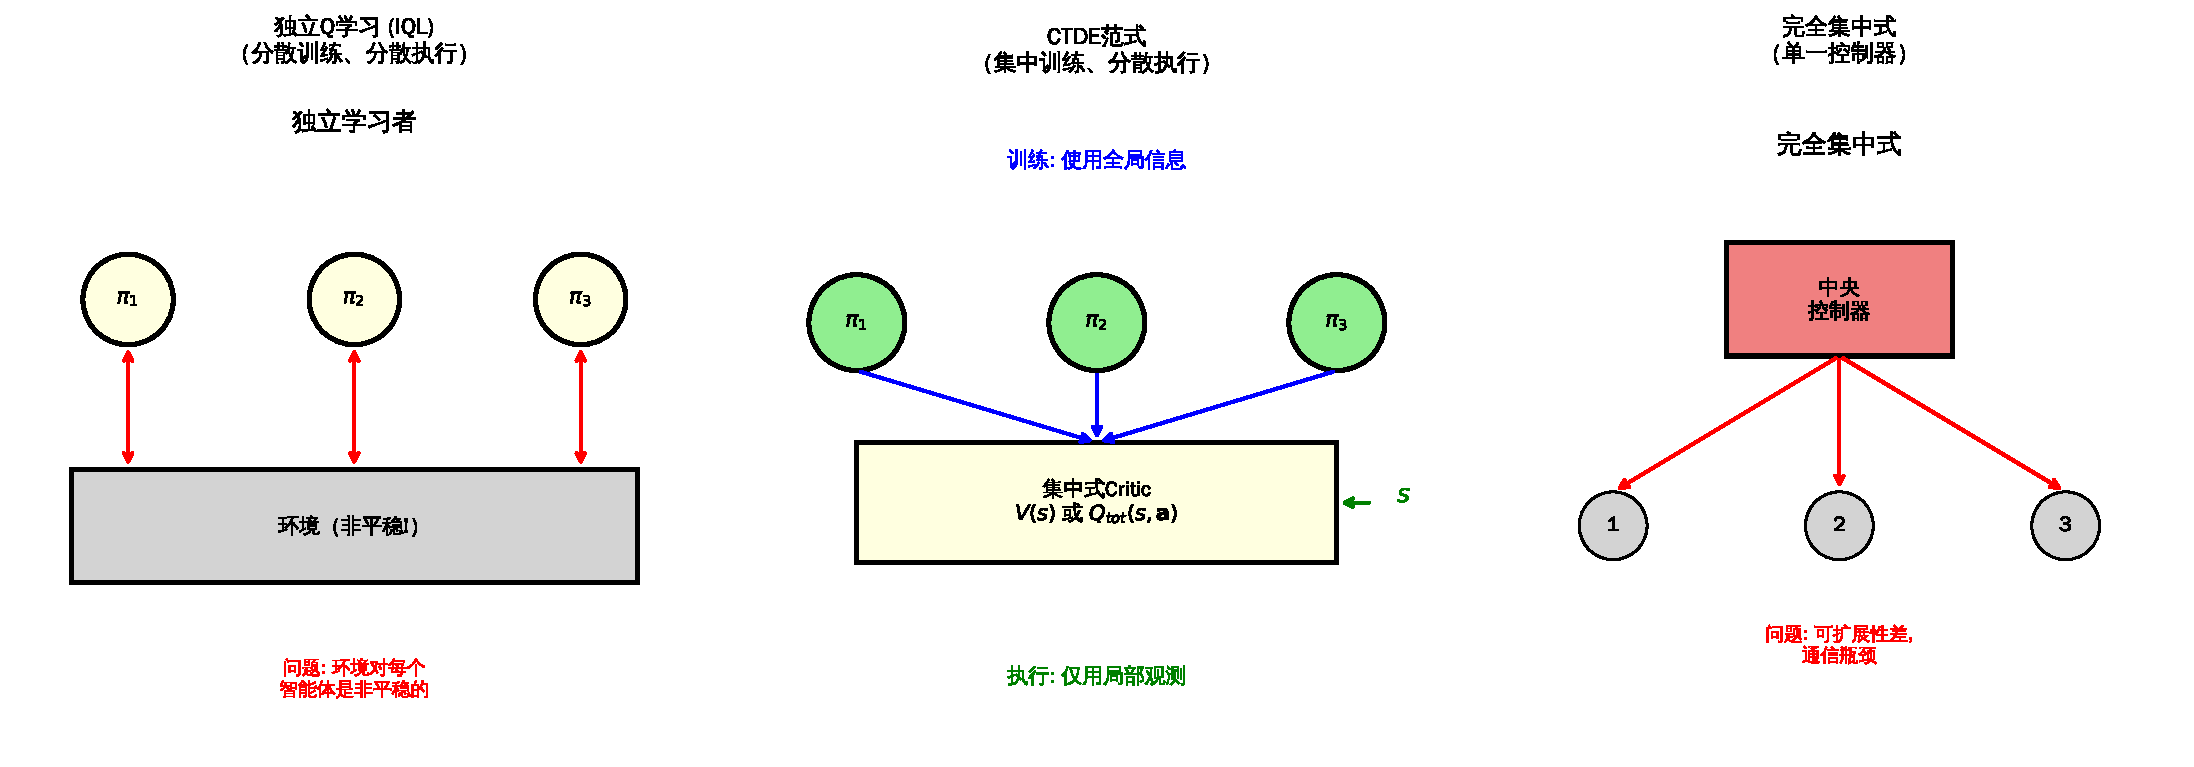
\includegraphics[width=0.95\textwidth]{figs_chap15/ctde_comparison.pdf}
\caption{三种多智能体学习范式的对比。左：独立学习（IQL），每个智能体独立与环境交互，面临非平稳性问题。中：CTDE范式，训练时使用全局信息（集中式Critic），执行时只用局部观测（分散式Actor）。右：完全集中式，由单一控制器指挥所有智能体，存在可扩展性和通信瓶颈问题。}
\label{fig:ctde}
\end{figure}

图\ref{fig:ctde}对比了三种学习范式。CTDE是目前最流行的方法，因为它在\textbf{训练效率}和\textbf{执行灵活性}之间取得了很好的平衡。

\subsection{价值分解方法：QMIX}

QMIX是CTDE范式下\textbf{价值分解}（Value Decomposition）方法的代表。

\begin{definition}[IGM原则——核心思想]
\textbf{IGM}（Individual-Global-Max）原则要求：
\begin{equation}
    \arg\max_{\mathbf{a}} Q_{tot}(s, \mathbf{a}) = \begin{pmatrix} \arg\max_{a_1} Q_1(o_1, a_1) \\ \vdots \\ \arg\max_{a_N} Q_N(o_N, a_N) \end{pmatrix}
\end{equation}

\textbf{直观理解}：最大化全局Q值的联合动作，等于每个智能体分别最大化自己局部Q值的动作组合。

\textbf{为什么重要}：这保证了分散执行的一致性——每个智能体贪婪地选择自己的最优动作，组合起来就是全局最优！
\end{definition}

\begin{theorem}[QMIX的单调性约束]
如果$Q_{tot}$关于每个$Q_i$是单调递增的：
\begin{equation}
    \frac{\partial Q_{tot}}{\partial Q_i} \geq 0, \quad \forall i
\end{equation}
则IGM原则自动满足。
\end{theorem}

\begin{proof}
设$a_i^* = \arg\max_{a_i} Q_i(o_i, a_i)$。

对于任意其他动作$a_i'$，有$Q_i(o_i, a_i^*) \geq Q_i(o_i, a_i')$。

由单调性（$Q_{tot}$ 对每个 $Q_i$ 非减），对任意联合动作 $a' = (a_1', \ldots, a_N')$，逐个坐标替换：
\begin{equation}
    Q_{tot}(s, a_1^*, a_2^*, \ldots, a_N^*) \geq Q_{tot}(s, a_1', a_2^*, \ldots, a_N^*) \geq Q_{tot}(s, a_1', a_2', \ldots, a_N^*) \geq \cdots \geq Q_{tot}(s, a')
\end{equation}
每一步只换一个坐标，用一次单调性。所以$(a_1^*, \ldots, a_N^*)$最大化$Q_{tot}$。
\end{proof}

\begin{figure}[htbp]
\centering
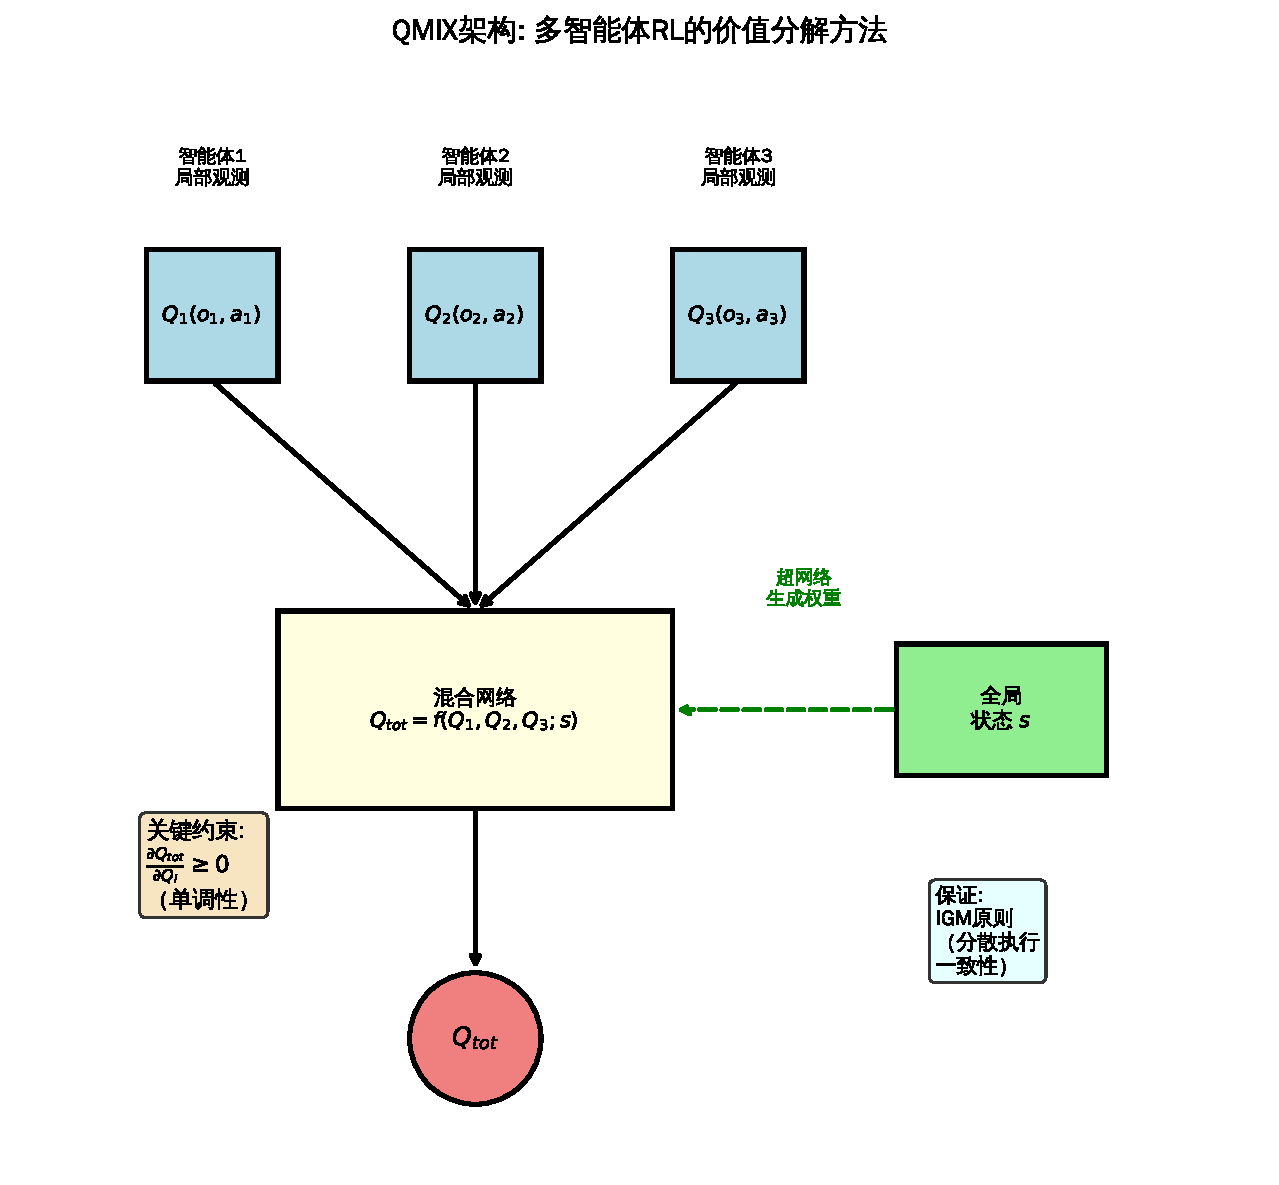
\includegraphics[width=0.8\textwidth]{figs_chap15/qmix_architecture.pdf}
\caption{QMIX架构示意图。每个智能体有自己的Q网络$Q_i(o_i, a_i)$，只使用局部观测。混合网络将各个局部Q值组合成全局Q值$Q_{tot}$。关键：混合网络的权重由超网络（Hypernetwork）根据全局状态$s$生成，且保证对$Q_i$的偏导非负（单调性约束），从而满足IGM原则。}
\label{fig:qmix}
\end{figure}

\textbf{QMIX架构的关键组件}（见图\ref{fig:qmix}）：
\begin{enumerate}
    \item \textbf{局部Q网络}：每个智能体$i$有一个Q网络$Q_i(o_i, a_i)$，只使用自己的观测
    \item \textbf{混合网络}：将所有局部Q值组合成全局Q值
    \item \textbf{超网络}：根据全局状态$s$生成混合网络的权重
    \item \textbf{非负权重}：通过绝对值或指数函数保证权重非负，从而满足单调性
\end{enumerate}

\begin{algorithm}
\caption{QMIX训练流程（伪代码）}
\begin{algorithmic}[1]
\State \textbf{输入}: 经验回放池，学习率$\alpha$，目标网络更新率$\tau$
\For{每个训练步}
    \State 从回放池采样一批经验 $(o, a, r, o', s, s', done)$
    \State \Comment{$o$: 各智能体观测, $a$: 各智能体动作, $s$: 全局状态}

    \State \textbf{计算当前Q值}:
    \For{每个智能体 $i$}
        \State $Q_i \leftarrow Q_i(o_i, a_i; \theta_i)$ \Comment{局部Q网络}
    \EndFor
    \State $Q_{tot} \leftarrow \text{MixingNetwork}(Q_1, \ldots, Q_N; s)$ \Comment{混合得到全局Q}

    \State \textbf{计算目标Q值}:
    \For{每个智能体 $i$}
        \State $Q'_i \leftarrow \max_{a'_i} Q^{target}_i(o'_i, a'_i)$ \Comment{目标网络}
    \EndFor
    \State $Q'_{tot} \leftarrow \text{MixingNetwork}^{target}(Q'_1, \ldots, Q'_N; s')$
    \State $y \leftarrow r + \gamma (1 - done) \cdot Q'_{tot}$ \Comment{TD目标}

    \State \textbf{更新网络}:
    \State $\mathcal{L} \leftarrow (Q_{tot} - y)^2$ \Comment{TD损失}
    \State 梯度下降更新所有网络参数
    \State 软更新目标网络: $\theta^{target} \leftarrow \tau \theta + (1-\tau) \theta^{target}$
\EndFor
\end{algorithmic}
\end{algorithm}

\begin{physicalintuition}
QMIX的单调性约束有深刻的物理意义：

\textbf{总能量是子系统能量的非线性叠加}。

想象一个物理系统由$N$个子系统组成，每个子系统有能量$E_i$。如果：
\begin{equation}
    \frac{\partial E_{tot}}{\partial E_i} \geq 0
\end{equation}

这意味着：任何子系统能量的增加都会导致总能量增加。没有"负能量贡献"。

QMIX假设的是一个\textbf{协作博弈}：每个智能体的"贡献"都是正向的。这在很多团队任务中是合理的（如星际争霸的微操、机器人协作搬运等）。

但如果智能体之间存在竞争关系（零和或混合博弈），QMIX的表达能力就不足了——这时需要其他方法。
\end{physicalintuition}

\subsection{策略梯度方法：MAPPO}

MAPPO是将PPO（近端策略优化）扩展到多智能体设置的方法。

\begin{definition}[MAPPO]
MAPPO使用Actor-Critic架构：
\begin{itemize}
    \item \textbf{Actor}（分散）：每个智能体$i$有自己的策略网络$\pi_i(a_i | o_i)$，只依赖局部观测
    \item \textbf{Critic}（集中）：一个共享的价值网络$V(s)$，使用全局状态
\end{itemize}

\review{第10章}{$L^{\text{CLIP}}$ 的来历见第10章扩展阅读"PPO：用裁剪代替约束"——它是把信赖域约束 $\mathrm{KL}(\pi_\theta \| \pi_{\theta_{\rm old}}) \le \delta$ 的拉格朗日形式换成一个便宜的替代品。}
策略更新使用PPO的裁剪目标：
\begin{equation}
    L^{\text{CLIP}}_i = \E\left[ \min\left( r_t(\theta) \hat{A}_t, \text{clip}(r_t(\theta), 1-\epsilon, 1+\epsilon) \hat{A}_t \right) \right]
\end{equation}
其中：
\begin{itemize}
    \item $r_t(\theta) = \frac{\pi_\theta(a_t | o_t)}{\pi_{\theta_{\text{old}}}(a_t | o_t)}$：新旧策略的概率比
    \item $\hat{A}_t$：优势函数估计（这个动作比平均好多少）
    \item $\epsilon$：裁剪参数（通常取0.1-0.2）
\end{itemize}
\end{definition}

\begin{remark}[MAPPO vs QMIX]
\begin{center}
\begin{tabular}{l|cc}
\toprule
& \textbf{QMIX} & \textbf{MAPPO} \\
\midrule
方法类型 & 价值分解 & 策略梯度 \\
动作空间 & 离散为主 & 离散/连续都可 \\
训练稳定性 & 较稳定 & 需要仔细调参 \\
表达能力 & 受单调性限制 & 更灵活 \\
适用场景 & 纯协作博弈 & 更广泛 \\
\bottomrule
\end{tabular}
\end{center}
\end{remark}

% ====================================================================================
\section{宏观极限：平均场博弈}
% ====================================================================================

\subsection{维度灾难与平均场近似}

当智能体数量很大时（如$N = 10000$个无人机、百万级的交通参与者），直接处理$N$体博弈面临\textbf{维度灾难}：
\begin{itemize}
    \item 联合状态空间：$\mathcal{S}^N$
    \item 联合动作空间：$\mathcal{A}^N$
    \item 存储和计算指数增长
\end{itemize}

\textbf{平均场近似}的思想来自统计物理：

\begin{quote}
\textit{当粒子数量趋于无穷时，忽略具体个体，只关注群体的统计分布。}
\end{quote}

\marginnote{\textbf{平均场博弈创始人}：MFG由法国数学家Jean-Michel Lasry和Pierre-Louis Lions于2006年合作提出；几乎同时，Huang、Malhamé 和 Caines 在加拿大独立提出了同样的思想。Lions是1994年菲尔兹奖得主（数学界最高荣誉），专长非线性PDE。他在法兰西公学院的MFG课程推动了该领域的蓬勃发展。}

\begin{definition}[平均场博弈]
在\textbf{平均场博弈}（Mean Field Game, MFG）中：
\begin{itemize}
    \item 有无穷多个同质（相同）智能体
    \item 每个智能体与群体分布$m(x, t)$交互，而不是与具体个体交互
    \item 群体分布由所有智能体的策略决定
\end{itemize}

\textbf{核心简化}：把``与$N$个具体对手的博弈''替换为``与群体分布的博弈''。
\end{definition}

\begin{example}[平均场近似的直观理解]
想象你是一滴水在大海中。

\textbf{微观视角}：你要考虑周围每一滴水的位置和速度（几乎不可能）

\textbf{平均场视角}：你只需要知道周围水的"平均流动方向"（密度场和速度场）

类似地，在有大量智能体的博弈中：
\begin{itemize}
    \item 你不需要知道每个对手的具体策略
    \item 你只需要知道对手群体的"分布"——有多少比例在做什么
    \item 基于这个分布，你做出最优响应
    \item 当每个人都这样做时，形成一个自洽的均衡
\end{itemize}
\end{example}

\subsection{MFG的核心思想：两步不动点}

理解MFG最关键的是把它看成一个\textbf{两步迭代过程}，最终要找的是一个\textbf{不动点}：

\begin{keyidea}[MFG的不动点结构——给大二同学的直观解释]
想象你是无数智能体中的一个，你需要做两件事：

\textbf{第一步：猜测别人的行为}

你不知道每个具体对手会做什么，但你可以``猜''一个群体分布$m(x,t)$——表示``在时刻$t$，有多少比例的智能体在位置$x$附近''。

\textbf{第二步：基于猜测，优化自己}

假设群体分布就是$m$，那么你面临的是一个\textbf{单人最优控制问题}——环境（别人的分布）已经固定了，你只需要最小化自己的代价。解这个问题得到\textbf{最优策略}$\pi^*(m)$和对应的\textbf{价值函数}$u(x,t)$。

\textbf{第三步：验证猜测是否自洽}

如果每个智能体都用$\pi^*(m)$这个策略，那么所有人的运动会产生一个新的密度分布$m'$。问题来了：$m'$和你最初猜的$m$一样吗？

\textbf{不动点条件}：如果$m' = m$，说明你的猜测是自洽的——每个人基于这个分布做最优决策，而这些最优决策恰好产生了这个分布。这就是\textbf{纳什均衡}！

\begin{center}
\begin{tikzpicture}[>=stealth, scale=0.9]
    \node[draw, rounded corners, fill=blue!15, minimum width=3cm, minimum height=1.2cm, align=center] (m) at (0, 0) {群体分布\\$m(x,t)$};
    \node[draw, rounded corners, fill=orange!15, minimum width=3cm, minimum height=1.2cm, align=center] (u) at (6, 0) {最优策略/价值函数\\$u(x,t), \pi^*$};

    \draw[->, thick] (m.east) -- node[above, font=\small] {固定$m$，解最优控制} node[below, font=\small, gray] {(HJB方程)} (u.west);
    \draw[->, thick] (u.south) .. controls (6, -2) and (0, -2) .. node[below, font=\small] {按$\pi^*$行动，推导密度} node[above, font=\small, gray] {(FP方程)} (m.south);

    \node[font=\small, red] at (3, -2.8) {\textbf{不动点}：$m \xrightarrow{\text{HJB}} u \xrightarrow{\text{FP}} m$};
\end{tikzpicture}
\end{center}
\end{keyidea}

\subsection{MFG的数学方程}

上面的直觉对应两个偏微分方程：

\begin{keyformula}[title=平均场博弈方程组]
\textbf{1. HJB方程}（``给定$m$，求最优策略''）：
\begin{equation}
    -\frac{\partial u}{\partial t} - \nu \Delta u + H(x, \nabla u, m) = 0, \quad u(x, T) = g(x), \qquad H(x, p, m) = \max_v \left[ -p \cdot v - L(x, v, m) \right]
\end{equation}
这是一个\textbf{后向方程}：从终端条件$g(x)$出发，往回算每个时刻的最优代价$u(x,t)$；$\nu \Delta u$ 项来自智能体受到的布朗运动扰动。
\review{第8章}{$u(x, t)$ 就是第8章的值函数 / 协态：HJB 从终端条件倒着算，和伴随方程"从未来往回算影响"是同一件事。这里的新意只在于 $H$ 里多了一个群体分布 $m$。}

\textbf{2. FP方程}（``给定最优策略，算密度演化''）：
\begin{equation}
    \frac{\partial m}{\partial t} + \nabla \cdot (m \cdot v^*) - \nu \Delta m = 0, \quad m(x, 0) = m_0(x)
\end{equation}
这是一个\textbf{前向方程}：从初始分布$m_0(x)$出发，根据最优速度场$v^* = -\nabla_p H$往前推演密度如何变化。

\textbf{耦合与不动点}：
\begin{itemize}
    \item HJB需要$m$：你的最优策略取决于别人在哪里（拥挤效应等）
    \item FP需要$u$：密度演化取决于大家的最优运动方向
    \item \textbf{纳什均衡} = 同时满足两个方程的$(u^*, m^*)$
\end{itemize}
\end{keyformula}

\begin{remark}[物理直觉]
\begin{itemize}
    \item \textbf{HJB方程}：类似量子力学中的Schrödinger方程，描述``价值波''的演化
    \item \textbf{FP方程}：就是连续性方程/扩散方程，描述概率密度的输运
\end{itemize}
MFG是统计力学和最优控制的交叉——群体行为的``热力学''。
\end{remark}

\begin{example}[线性二次MFG——一个可以精确求解的例子]
为了让上面的抽象方程变得具体，我们考虑一个最简单的MFG问题：

\textbf{场景}：无穷多个智能体在一维空间$x \in \mathbb{R}$上运动，时间$t \in [0, T]$。

\textbf{每个智能体的目标}：最小化自己的代价
\begin{equation}
    J = \int_0^T \left[ \frac{1}{2}v^2 + \frac{\alpha}{2}(x - \bar{x})^2 \right] dt + \frac{1}{2}x(T)^2
\end{equation}
其中：
\begin{itemize}
    \item $\frac{1}{2}v^2$：控制代价——速度越大，``油费''越贵
    \item $\frac{\alpha}{2}(x - \bar{x})^2$：\textbf{跟随代价}——$\alpha > 0$ 时希望靠近群体平均位置$\bar{x} = \int x \, m(x,t) dx$（$\alpha < 0$ 则变成拥挤代价，越远越好）
    \item $\frac{1}{2}x(T)^2$：终端代价——最后希望靠近原点
\end{itemize}

\textbf{动力学}：每个智能体按$\dot{x} = v$运动，并受布朗运动扰动（扩散系数$\nu$）。

\textbf{初始条件}：所有智能体初始集中在原点附近，$m_0(x) \sim \mathcal{N}(0, \sigma_0^2)$。

这个问题的MFG方程可以用有限差分法数值求解：HJB 从 $T$ 往回算、FP 从 $0$ 往前算，交替迭代直到不动点。图\ref{fig:mfg}就是这样算出来的一个\textbf{真实数值解}——为了让``别人对我的价格''看得见，图中把跟随代价换成了\textbf{拥挤代价}：$F(x,m)=\frac{\alpha}{2}(x-x_{\rm target})^2+\kappa\, m(x,t)$（想去目标点 $x_{\rm target}=1$，但当地人越多越贵），群体从 $x\approx-1$ 出发，终端代价 $g(x)=\frac{\alpha}{2}(x-x_{\rm target})^2$，参数 $\alpha=3$、$\kappa=2$、$\nu=0.05$、$T=1.5$。
\end{example}

\begin{figure}[htbp]
\centering
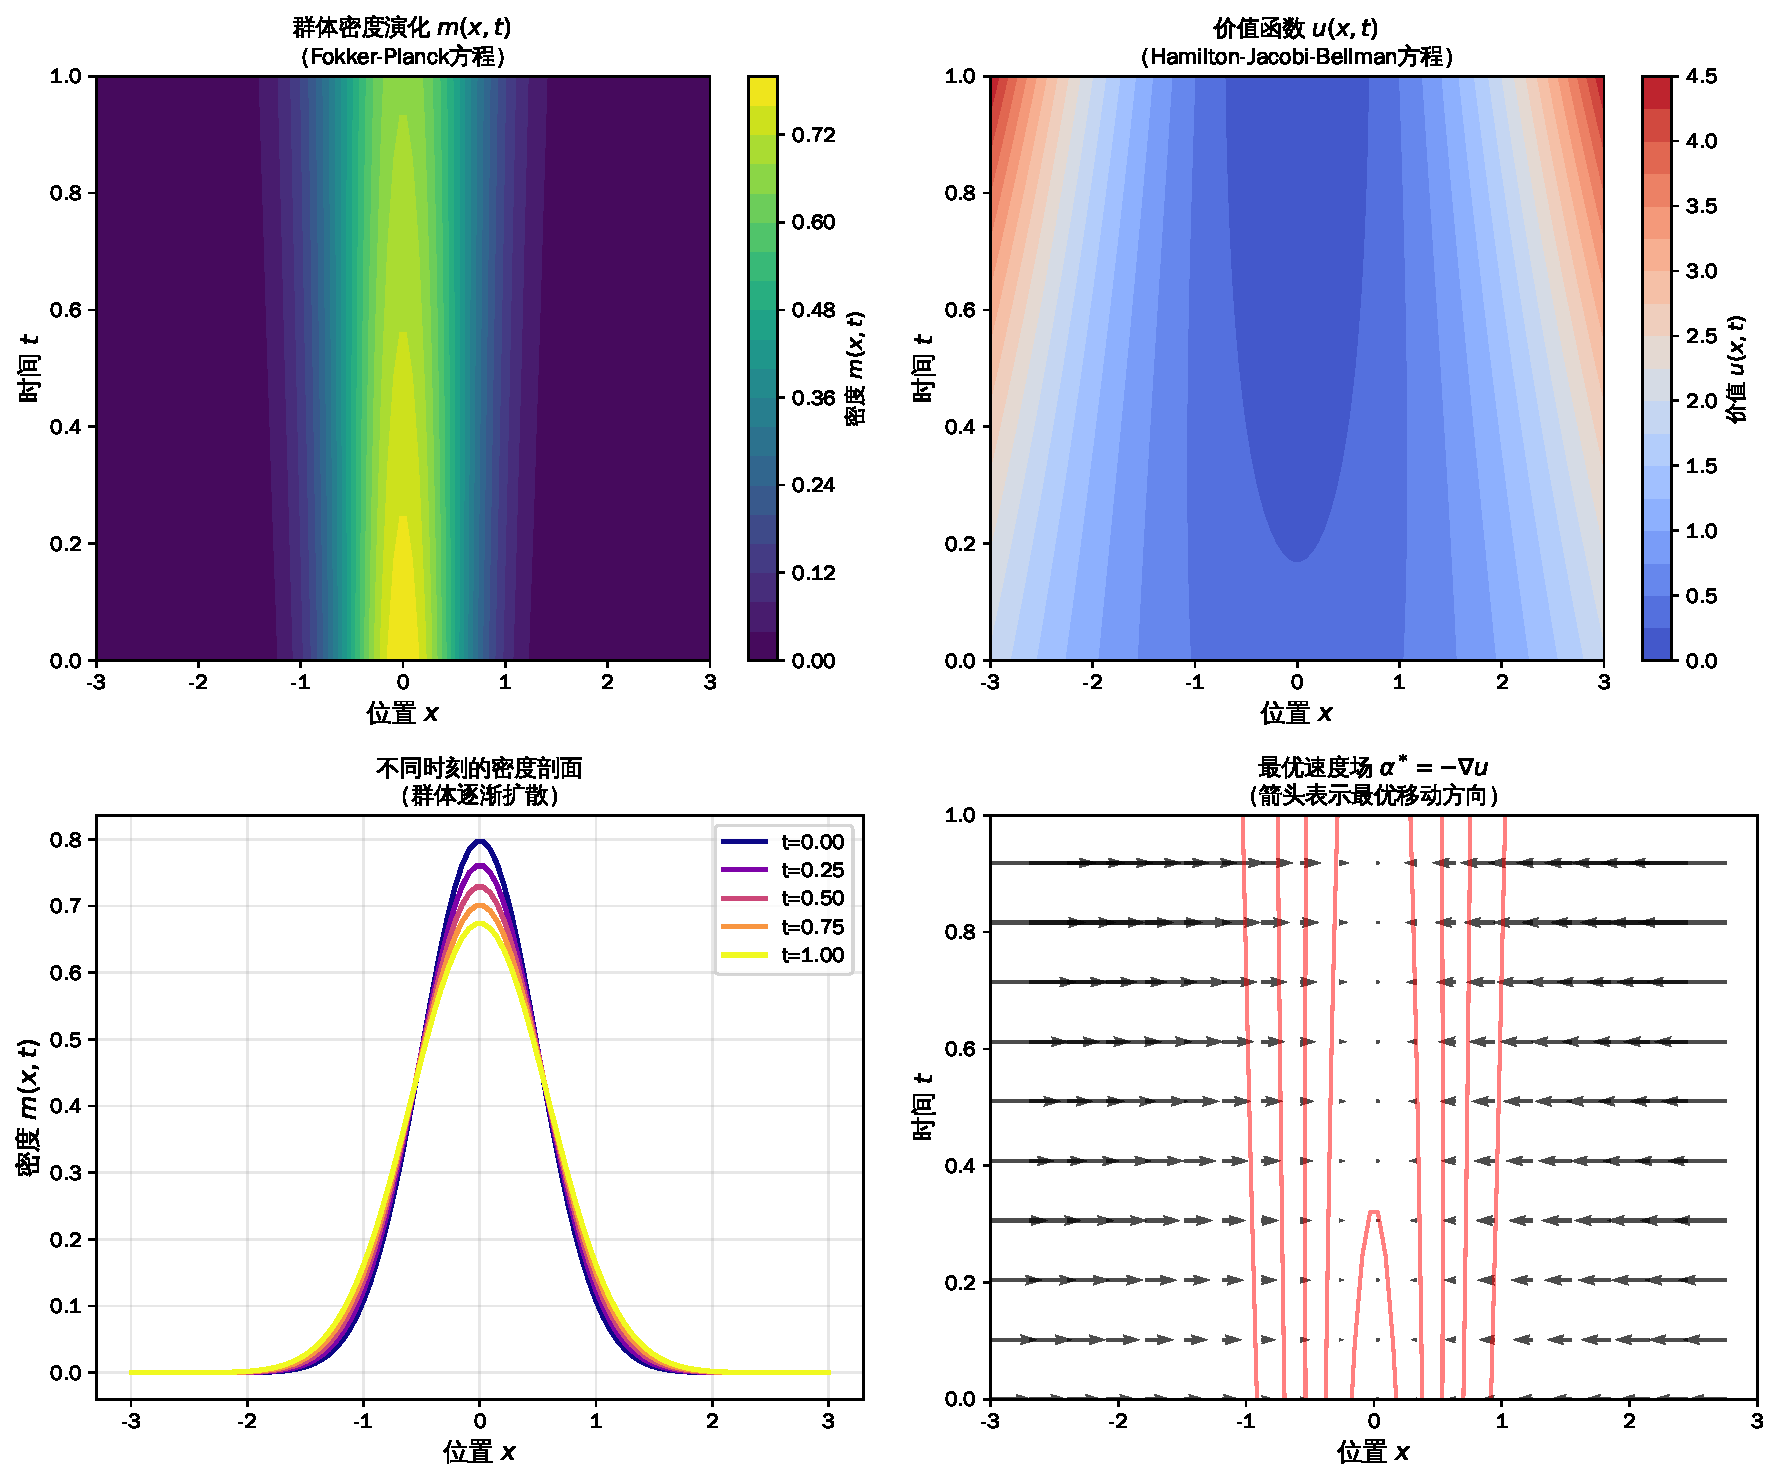
\includegraphics[width=0.95\textwidth]{figs_chap15/mfg_solution.pdf}
\caption{一维平均场博弈的数值解（有限差分 + 阻尼不动点迭代，代码 \texttt{code\_chap15/chap15\_mfg\_solver.py}）。每个人的运行代价是 $\frac12 v^2+\frac{\alpha}{2}(x-x_{\rm target})^2+\kappa\, m(x,t)$：想去目标点 $x_{\rm target}=1$（黑色点线），但讨厌拥挤。(a) 密度 $m(x,t)$：群体从 $x=-1$ 整体迁往目标点；红色虚线是沿最优速度场 $\dot x=-\partial_x u$ 积分出的个体轨迹——个体随群体一起走，但走在最前面的人会越过目标点，给后面的人让位。(b) 价值函数 $u(x,t)$（离目标越远代价越高）与最优速度 $v^*=-\partial_x u$（箭头）：$u$ 就是第8章的协态、本章的 $\lambda$，它的梯度直接告诉每个人该往哪走、走多快。(c) 不同时刻的密度剖面：有拥挤惩罚（$\kappa=2$）时，$t=T$ 的群体铺成峰值 $1.3$、标准差 $0.28$ 的宽平台；把 $\kappa$ 设为 $0$（灰色虚线）群体就挤成峰值 $2.6$、标准差 $0.16$ 的尖峰。(d) 不动点迭代残差：$m\to$HJB$\to u\to$FP$\to\tilde m$ 每一轮的变化量按指数衰减，约 110 轮后降到 $10^{-8}$——$(u^*,m^*)$ 确实是自洽的纳什均衡，不是画出来的。}
\label{fig:mfg}
\end{figure}

\textbf{从图中可以观察到}：
\begin{itemize}
    \item \textbf{(a)}：群体整体从 $x=-1$ 迁往目标点，但并不是每个人都停在目标点上——个体轨迹在 $t=T$ 时分散在 $x\approx0.5$ 到 $1.3$ 之间，前面的人越过目标点给后面的人让位。这就是拥挤代价 $\kappa m$ 在起作用：它是群体分布 $m$ 反过来施加给每个个体的``价格''
    \item \textbf{(b)}：价值函数在离目标远的地方最大（深色），越靠近目标越平缓；最优速度 $v^*=-\partial_x u$ 在目标点两侧相向指向目标，靠近目标后箭头变短——个体只按自己所在位置的 $\nabla u$ 行动，不需要知道别人的具体位置，这正是平均场近似的含义
    \item \textbf{(c)}：把 $\kappa$ 从 $2$ 调到 $0$，$t=T$ 的密度从宽平台变成尖峰。拥挤惩罚让个体宁可离目标远一点也要避开人群，宏观上就是群体``摊开''
    \item \textbf{(d)}：HJB 需要 $m$、FP 需要 $u$，两者互为约束；纳什均衡是这对方程组的不动点，残差按指数衰减到 $10^{-8}$ 说明它被真正算出来了（迭代时要加阻尼 $m\leftarrow(1-\theta)m+\theta\tilde m$，否则``人多的地方大家都想离开''会让迭代来回振荡）
\end{itemize}

% ====================================================================================
\section{本章小结}
% ====================================================================================

\begin{enumerate}
    \item \textbf{从优化到博弈}：单人优化只有一个决策者；多人博弈里每个人的最优依赖于他人的选择。纳什均衡是"没有人想单方面改变"的稳定状态。
    \item \textbf{静态博弈的分析工具}：广义纳什均衡 = 所有玩家的 KKT 条件同时成立；势博弈的自私行为恰好在优化一个全局势函数（保证收敛）；图博弈只有局部交互，可分布式计算；Braess 悖论说明增加选择反而可能让所有人更差。
    \item \textbf{动态博弈与深度 MARL}：CTDE 范式集中训练、分散执行；QMIX 用单调性约束保证 IGM；MAPPO 用集中式 Critic + 分散式 Actor。
    \item \textbf{宏观极限——平均场博弈}：$N \to \infty$ 时多体交互变成个体--场交互，HJB（后向）+ FP（前向）耦合方程组把博弈论接到了偏微分方程与统计物理。
\end{enumerate}

\begin{physicalmeaning}
\textbf{$\lambda$ 在本章的意义}：
\begin{itemize}
    \item \textbf{玩家自己的约束}：$\lambda_{ij}$ 是玩家 $i$ 为放松第 $j$ 条约束愿意付出的代价——第1章的影子价格原封不动，只是每人各有一份。
    \item \textbf{交通均衡}：需求约束的乘子 $\lambda_w = \partial \Phi^*/\partial d_w$ 等于均衡旅行时间；非负约束的乘子 $\mu_p$ 是路径 $p$ 比最短路"慢多少"。把 $t_a$ 换成边际社会成本后，多出来的 $x_a t_a'(x_a)$ 就是拥堵费。
    \item \textbf{平均场极限}：值函数 $u(x, t)$ 是 $\lambda$ 的连续版本（第8章的协态），$\nabla u$ 直接给出每个人的最优速度。
\end{itemize}
第4章 $\lambda$ = 约束力，第8章 $\lambda(t)$ = 伴随变量，第10章 $\lambda$ = 值函数梯度；本章它变成了"别人对我的价格"。下一章（第16章）它将以"安全约束的斥力"再次出现。
\end{physicalmeaning}

\begin{unification}[title=从微观到宏观的统一视角]
\begin{center}
\begin{tabular}{lccc}
\toprule
\textbf{维度} & \textbf{微观} & \textbf{中观} & \textbf{宏观} \\
\midrule
\textbf{智能体数} & 少量（2-10） & 中等（10-1000） & 无穷 \\
\textbf{核心对象} & 个体动作 $a_i$ & 联合动作 $\mathbf{a}$ & 密度分布 $m(x)$ \\
\textbf{静态模型} & 纳什均衡 & 图博弈/势博弈 & Wardrop均衡 \\
\textbf{动态模型} & 两人马尔可夫博弈 & Markov Game & MFG (HJB-FP) \\
\textbf{AI算法} & 自博弈（AlphaZero） & QMIX/MAPPO & Neural MFG \\
\textbf{物理类比} & 质点力学 & 多体系统 & 流体力学/统计物理 \\
\bottomrule
\end{tabular}
\end{center}

这个表格展示了一个美妙的对应：随着智能体数量的增加，我们从离散的个体视角逐渐过渡到连续的场视角，就像从牛顿力学过渡到流体力学一样。
\end{unification}

% ====================================================================================
\section{习题}
% ====================================================================================

\paragraph{计算题}
\begin{enumerate}
    \item \textbf{纳什均衡的理解}：
    考虑以下"协调博弈"：两个人要选择在哪里见面，可以选A地或B地。如果选同一个地方就能见面（代价0），选不同地方就见不到（代价1）。
    \begin{enumerate}
        \item 写出代价矩阵
        \item 找出所有纳什均衡
        \item 解释为什么会有多个纳什均衡
        \item 这个博弈是势博弈吗？为什么？
    \end{enumerate}
    
    \item \textbf{Braess悖论的变种}：
    在Braess悖论的例子中，如果免费道路AB的时间不是0，而是一个正数$c$，问：
    \begin{enumerate}
        \item $c$取什么范围时，悖论仍然存在（有免费道路更差）？
        \item $c$取什么值时，有道路和没道路的均衡时间相同？
        \item 给出直观解释。
    \end{enumerate}
    
    \item \textbf{图博弈的KKT条件}：
    对于代价函数$J_i = \frac{1}{2}(a_i - a_{i,0})^2 + \delta a_i \sum_{j \in N(i)} a_j$和约束$a_i \in [0, L]$：
    \begin{enumerate}
        \item 写出每个玩家的拉格朗日函数（提示：需要两个乘子，分别对应$a_i \geq 0$和$a_i \leq L$）
        \item 推导KKT条件
        \item 证明投影最优响应$a_i = \Pi_{[0,L]}(a_{i,0} - \delta \sum_{j} a_j)$满足KKT条件
        \item 其中$\Pi_{[0,L]}(x) = \max(0, \min(x, L))$是到区间$[0,L]$的投影
    \end{enumerate}
    
\end{enumerate}

\paragraph{证明题}
\begin{enumerate}
    \setcounter{enumi}{3}
    \item \textbf{QMIX的IGM证明}：
    证明：如果$\frac{\partial Q_{tot}}{\partial Q_i} \geq 0$对所有$i$成立，则IGM原则满足。
    
    提示：用反证法，假设存在$a'$使得$Q_{tot}(s, a') > Q_{tot}(s, a^*)$，其中$a_i^* = \arg\max Q_i$，推导矛盾。
    
\end{enumerate}

\paragraph{编程题}
\begin{enumerate}
    \setcounter{enumi}{4}
    \item \textbf{实现迭代最优响应}：
    对于例\ref{ex:lq_network}中的线性二次图博弈：
    \begin{enumerate}
        \item 用Python实现迭代最优响应算法
        \item 在一个10节点的随机图上测试收敛性
        \item 画出收敛曲线，验证线性收敛率
        \item 探索：$\delta$取什么值时算法不收敛？与图的谱半径有什么关系？
    \end{enumerate}
    
    \item \textbf{Braess悖论的数值验证}：
    参考本章的Python代码（\texttt{chap15\_generate\_figures.py}）：
    \begin{enumerate}
        \item 复现Braess悖论的计算
        \item 修改需求量（从4000变为其他值），观察悖论是否仍然存在
        \item 设计一个你自己的交通网络，尝试找到/构造Braess悖论
    \end{enumerate}
    
\end{enumerate}

\paragraph{思考题}
\begin{enumerate}
    \setcounter{enumi}{6}
    \item Wardrop 均衡的乘子 $\lambda_w$ 是均衡旅行时间。如果政府按边际社会成本 $x_a t_a'(x_a)$ 对每条路收拥堵费，新的均衡会变成什么？它和"系统最优"是什么关系？谁受益、谁受损？
    
    \item 第2章把拉格朗日函数看成 $x$ 与 $\lambda$ 的零和博弈。本章的势博弈是"$N$ 组 KKT 恰好是同一个函数的 KKT"。两者有什么共同点？一个非零和博弈什么时候会退化成单人优化？
\end{enumerate}

% ====================================================================================
\section*{扩展阅读：延伸文献}
\addcontentsline{toc}{section}{扩展阅读：延伸文献}
% ====================================================================================

\begin{enumerate}
    \item \textbf{博弈论入门}：Osborne, M. J. (2004). \textit{An Introduction to Game Theory}. Oxford University Press. 非常适合本科生的博弈论教材。

    \item \textbf{平均场博弈}：Lasry, J. M., \& Lions, P. L. (2007). Mean field games. \textit{Japanese Journal of Mathematics}, 2(1), 229-260. 平均场博弈的奠基性论文。

    \item \textbf{QMIX}：Rashid, T., et al. (2018). QMIX: Monotonic value function factorisation for deep multi-agent reinforcement learning. \textit{ICML 2018}. 价值分解方法的里程碑。

    \item \textbf{MAPPO}：Yu, C., et al. (2022). The surprising effectiveness of PPO in cooperative multi-agent games. \textit{NeurIPS 2022}. 展示了简单方法在多智能体RL中的强大能力。

    \item \textbf{Braess悖论}：Braess, D. (1968). Über ein Paradoxon aus der Verkehrsplanung. \textit{Unternehmensforschung}, 12(1), 258-268. 原始论文（德语）。

    \item \textbf{交通均衡}：Wardrop, J. G. (1952). Road paper. Some theoretical aspects of road traffic research. \textit{Proceedings of the Institution of Civil Engineers}, 1(3), 325-362. 交通均衡理论的经典。
\end{enumerate}
